\documentclass{exerciseBlue}

\settitle[Zusammenfassung]{Medical Robotics}
\addstudent[653897]{Alexander Osiik}
\usepackage{tikz}
\usepackage{pifont}
\usepackage{pgf}
\usepackage{graphicx}
\usepackage{listings}
\usetikzlibrary{positioning}
\usetikzlibrary{arrows,  automata, fit, shapes}
\usetikzlibrary{matrix}
\tikzstyle{mycircle }=[circle, draw, thick]
\tikzstyle{myrect }=[ circle ,draw ,thick]

\begin{document}
	\section{Applications of Medical Robotics}
	 There are 4 types of Robots
	  \begin{itemize}
	  	\item Robots for \textbf{Navigation}\ref{sec:navigation}\\
	  	\textit{Surgical drill} for Precise positioning, motion compensation..
	  	\item Robots for \textbf{Imaging}\\
	  	\textit{Minimally-invasive surgery} by Motion downscaling, reduce tremor...
		\item Robots for \textbf{Motion Replication}\\
		\textit{Robotic ultrasound} for Automation, speed...
		\item \textbf{Rehabilitation} and \textbf{Prosthetics}\\
		\textit{Exoskeletons} that Replace damaged structures, autonomous rehabilitation...
	  \end{itemize}
	  Application: Epiphyseolysis
  
  \section{Navigation}\label{sec:navigation}
  \subsection{Problem: We have an image.}
  \begin{itemize}
  	\item  Where is the \textbf{Robot} in the image coordinate system?
  	\item Where is the \textbf{Target} in the image?
  \end{itemize}  
\subsection{Ingridients for Radiologic Navigation:}
\begin{itemize}
	\item \textbf{C-Arm Robot:}\\
	A mobile x-ray system, robot containing 2 prismatic and 3 revolute Joints
	\item \textbf{Infrared Tracking:}\\
	Place Marker on Endeffector, on Target and on C-Arm. A Camera the ncalculates the positions:
	\begin{itemize}
		\item Skin incision
		\item Place marker on bone
		\item Take 2 C-Arm images
		\item Tavigate
	\end{itemize}
	\item[$\implies$] Navigation, Registration, Calibration!
\end{itemize}
\subsection{Spatial position and orientation}
Every Transformation is a multiplication, simply write down the vectors.\\
Rotatory Matrices:\\
$R(x,\theta) = \begin{pmatrix}
1&0&0&0\\
0&C_{\theta}&-S_{\theta}&0\\
0&S_{\theta}&C_{\theta}&0\\
0&0&0&1
\end{pmatrix}, \ 
R(y,\theta) = \begin{pmatrix}
C_{\theta}&0&S_{\theta}&0\\
0&1&0&0\\
-S_{\theta}&0&C_{\theta}&0\\
0&0&0&1
\end{pmatrix}, \ 
R(z,\theta) = \begin{pmatrix}
C_{\theta}&-S_{\theta}&0&0\\
S_{\theta}&C_{\theta}&0&0\\
0&0&1&0\\
0&0&0&1
\end{pmatrix}$\\
Translatory Matrices:\\
$T(x,a) = \begin{pmatrix}
1&0&0&a\\
0&1&0&0\\
0&0&1&0\\
0&0&0&1
\end{pmatrix}, \ 
T(y,a) = \begin{pmatrix}
1&0&0&0\\
0&1&0&a\\
0&0&1&0\\
0&0&0&1
\end{pmatrix}, \ 
T(z,a) = \begin{pmatrix}
1&0&0&0\\
0&1&0&0\\
0&0&1&a\\
0&0&0&1
\end{pmatrix}$
\subsection{Denavit Hartenberg Parameter}
TODO
\\
In \textbf{Forward Kinematics}, we derive the Endeffector Position by multiplication of given Joint Matrices, e.g.\\
$$^BM_G = ^BM_1 \cdot  ^1M_2 \cdot  ^2M_3 \cdot  ^3M_G$$
In \textbf{Reverse Kinematics}, we calculate the Joint angles from a given Endeffector Position, e.g. One Joint Robot:\\
$P = (P_X, P_Y), \ \text{Get Angle } \theta \text{ by:} \dfrac{P_Y}{P_X} = \dfrac{\sin \theta}{\cos \theta} = \tan \theta \implies \theta = atan2(P_Y, P_X)$\\
Use atan2-Function, as it gives back the angles of full circle depending on signs 
  \section{Navigation \& Registration}
  \subsection{Problem: We have >1 images.}
  \begin{itemize}
  	\item Rotate images in such way, that images align
  	\item Output is $\theta, \triangle x, \triangle y$
    \end{itemize}
There are various types of Registration:
\begin{itemize}
	\item point-based
	\item landmark-based
	\item contour-based
	\item intensity-based
	\item elastic
\end{itemize}
\subsection{Landmark based registration}
Situation: We have an MR image of a head. We place 4 Landmarks (Nose and Mouth). The Target Point is given with respect to the four landmark points. \\
From this, two point clouds $A,B$ are generated.\\
We assume: $\#A = \#B, \ 2D, \ a_1\rightarrow b_1 \ etc.$\\
If we move $B$, this leads to:\\\\
$b_1 \leadsto R\cdot b_1 + t$, $R = \begin{pmatrix}
	\cos \theta & -\sin\theta\\
	\sin\theta & \cos\theta
\end{pmatrix}, t = \begin{pmatrix}
t_x\\
t_y
\end{pmatrix}$\\
$b_2 \leadsto R\cdot b_2 + t$\\
$\vdots$\\
$b_n \leadsto R\cdot b_n + t$\\\\
We create a function $f$, which is the distance between the two point clouds $A$ and $B$. We want to minimize this function:
$$f = ||R\cdot b_1 + t - a_1||^2+\dots+||R\cdot b_n + t - a_n||^2$$
\subsection{Gaussian Least Square}
If we assume that the angle $\theta$ is small, we can linearize the rotational matrix R such that:
$$\cos \theta \sim 1, \ \sin \theta \sim \theta \implies R = \begin{pmatrix}
1 & -\theta\\
\theta & 1
\end{pmatrix}$$\\
This matrix $R$ is linear in $\theta$.\\
We can also linearize the 3D rotation matrix as follows:
$$R(x,\alpha)\cdot R(y,\beta)\cdot R(z,\gamma) = \begin{pmatrix}
1 & \gamma & -\beta\\
-\gamma & 1 & \alpha\\
\beta & \alpha & 1
\end{pmatrix}$$
As the multiplication of two small values leads to an even smaller value. This method works fine until angles of 10 degrees.
\subsection{Iterative Closest Points (ICP)}
 Assume we have a point cloud $A$ and a point cloud $ B$. We want know the transformation needed to overlap $B$ over $A$. We do \textbf{not} deform $B$, as all motion is rigid (rotation and translation).\\
 Cloud A: 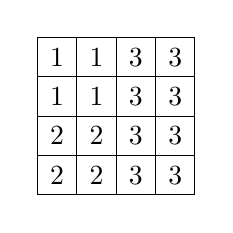
\begin{tikzpicture}
 \tikzset{square matrix/.style={
 		matrix of nodes,
 		column sep=-\pgflinewidth, row sep=-\pgflinewidth,
 		nodes={draw,
 			minimum height=#1,
 			anchor=center,
 			text width=#1,
 			align=center,
 			inner sep=0pt
 		},
 	},
 	square matrix/.default=.5cm
 }
 %|[fill=yellow]|
 \matrix[square matrix]
 {
 	1 & 1 & 3 & 3 \\
 	1 & 1 & 3 & 3 \\
 	2 & 2 & 3 & 3 \\
 	2 & 2 & 3 & 3 \\
 }; 
 \end{tikzpicture}
 Cloud B
  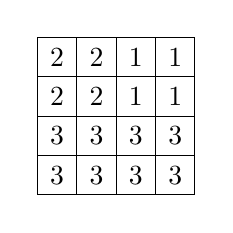
\begin{tikzpicture}
 
 \tikzset{square matrix/.style={
 		matrix of nodes,
 		column sep=-\pgflinewidth, row sep=-\pgflinewidth,
 		nodes={draw,
 			minimum height=#1,
 			anchor=center,
 			text width=#1,
 			align=center,
 			inner sep=0pt
 		},
 	},
 	square matrix/.default=.5cm
 }
 %|[fill=yellow]|
 \matrix[square matrix]
 {
 	2 & 2 & 1 & 1 \\
 	2 & 2 & 1 & 1 \\
 	3 & 3 & 3 & 3 \\
 	3 & 3 & 3 & 3 \\
 }; 
 \end{tikzpicture}
 $\implies $ Just rotate $90^o$ to align\\
 But sometimes, coloring differs in images depending on the imaging process. For Example, in CT the bone has a bright white color, while in MR the bone is more gray:\\
  Cloud A: 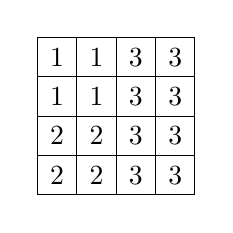
\begin{tikzpicture}
 \tikzset{square matrix/.style={
 		matrix of nodes,
 		column sep=-\pgflinewidth, row sep=-\pgflinewidth,
 		nodes={draw,
 			minimum height=#1,
 			anchor=center,
 			text width=#1,
 			align=center,
 			inner sep=0pt
 		},
 	},
 	square matrix/.default=.5cm
 }
 %|[fill=yellow]|
 \matrix[square matrix]
 {
 	1 & 1 & 3 & 3 \\
 	1 & 1 & 3 & 3 \\
 	2 & 2 & 3 & 3 \\
 	2 & 2 & 3 & 3 \\
 }; 
 \end{tikzpicture}
 Cloud B
 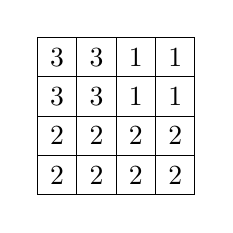
\begin{tikzpicture}
 
 \tikzset{square matrix/.style={
 		matrix of nodes,
 		column sep=-\pgflinewidth, row sep=-\pgflinewidth,
 		nodes={draw,
 			minimum height=#1,
 			anchor=center,
 			text width=#1,
 			align=center,
 			inner sep=0pt
 		},
 	},
 	square matrix/.default=.5cm
 }
 %|[fill=yellow]|
 \matrix[square matrix]
 {
 	3 & 3 & 1 & 1 \\
 	3 & 3 & 1 & 1 \\
 	2 & 2 & 2 & 2 \\
 	2 & 2 & 2 & 2 \\
 }; 
 \end{tikzpicture}
 $\implies $ rotate $90^o$ enough?\\
\subsection{Mutual Information (MI)}
For \textbf{Mutual Information} Registration, the color mapping does not have to be exactly 1x1. It can be different, as shown in the example above.\\
\textbf{Basic Definition:}\\
We generate Images $A,B$ in a random process. For each pixel of the image, we throw a dice (random generation), so we map 6 colors $\{1,\dots,6\}$ to each pixel. $A,B$ are random variables with distributions $P_A, P_B$, namely:
\begin{itemize}
	\item $P_A(a) = $ Probability of grey level value $a$ in image $A$ 
	\item $P_B(b) = $ Probability of grey level value $b$ in image $B$
	\item[$\implies$] $P_{A,B}(a,b) = $ Probability of grey level value $a$ in image $A$ occuring at the same position in image $B$ 
\end{itemize} 
Examples:
\begin{itemize}
	\item $A \neq B:$ $A$ tells nothing about $B$, 2 different images
	\item $A = B: $ $A$ tells everything about $B$ 
	\item $A$ tells something about $B$
\end{itemize}
Keep in mind the law of Independence of two random variables:
$$P_{A,B}(a,b) = P_A(a)\cdot P_B(b)$$
We want to know the maximum Mutual Information, calculated as follows:\\
$$I(A,B) = \sum_{a,b}P_{A,B}(a,b)\cdot \log_2 \left(\dfrac{P_{A,B}(a,b)}{P_A(a)\cdot P_B(b)}\right)$$
The Sum ranges over all greyscale pairs of diefferent colors. $I(A,B)$ measures the information dependencies. We maximize the Mutual Information to find exact position.\\
Example 1:$$A = 
 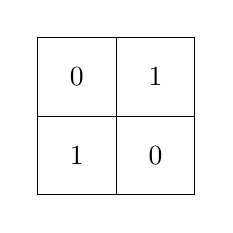
\begin{tikzpicture}

\tikzset{square matrix/.style={
		matrix of nodes,
		column sep=-\pgflinewidth, row sep=-\pgflinewidth,
		nodes={draw,
			minimum height=#1,
			anchor=center,
			text width=#1,
			align=center,
			inner sep=0pt
		},
	},
	square matrix/.default=1cm
}
%|[fill=yellow]|
\matrix[square matrix]
{
	0 & 1 \\
	1 & 0  \\
}; 
\end{tikzpicture}, \ \ B = 
 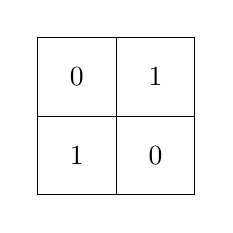
\begin{tikzpicture}

\tikzset{square matrix/.style={
		matrix of nodes,
		column sep=-\pgflinewidth, row sep=-\pgflinewidth,
		nodes={draw,
			minimum height=#1,
			anchor=center,
			text width=#1,
			align=center,
			inner sep=0pt
		},
	},
	square matrix/.default=1cm
}
%|[fill=yellow]|
\matrix[square matrix]
{
	0 & 1 \\
	1 & 0  \\
}; 
\end{tikzpicture}$$
$$P_A(0) = 0.5, \ P_B(0) = 0.5$$
$$P_A(1) = 0.5, \ P_B(1) = 0.5$$
$$P_{A,B}(0,0) = 0.5, \ P_{A,B}(0,1) = 0$$
$$P_{A,B}(1,1) = 0.5, \ P_{A,B}(1,0) = 0$$
$$\sum = 1$$
$$I(A,B) = \sum_{a,b}P_{A,B}(a,b)\cdot \log_2 \left(\dfrac{P_{A,B}(a,b)}{P_A(a)\cdot P_B(b)}\right)$$
$$= 0.5 \cdot \log_2 \left(\dfrac{P_{A,B}(0,0)}{P_A(0)\cdot P_B(0)}\right) + 0.5\cdot \log_2 \left(\dfrac{P_{A,B}(1,1)}{P_A(1)\cdot P_B(1)}\right) + 0\cdot \log_2 \left(\dfrac{P_{A,B}(0,1)}{P_A(0)\cdot P_B(1)}\right) + 0\cdot \log_2 \left(\dfrac{P_{A,B}(1,0)}{P_A(1)\cdot P_B(0)}\right)$$
$$= 0.5 \cdot \log_2 (2) + 0.5 \cdot \log_2(2)$$
$$= 1$$
Example 2:$$A = 
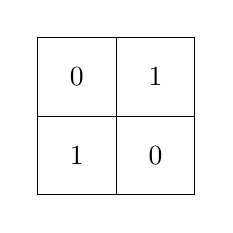
\begin{tikzpicture}

\tikzset{square matrix/.style={
		matrix of nodes,
		column sep=-\pgflinewidth, row sep=-\pgflinewidth,
		nodes={draw,
			minimum height=#1,
			anchor=center,
			text width=#1,
			align=center,
			inner sep=0pt
		},
	},
	square matrix/.default=1cm
}
%|[fill=yellow]|
\matrix[square matrix]
{
	0 & 1 \\
	1 & 0  \\
}; 
\end{tikzpicture}, \ \ B = 
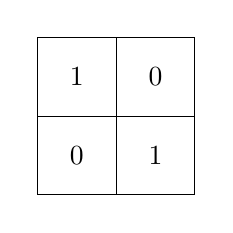
\begin{tikzpicture}

\tikzset{square matrix/.style={
		matrix of nodes,
		column sep=-\pgflinewidth, row sep=-\pgflinewidth,
		nodes={draw,
			minimum height=#1,
			anchor=center,
			text width=#1,
			align=center,
			inner sep=0pt
		},
	},
	square matrix/.default=1cm
}
%|[fill=yellow]|
\matrix[square matrix]
{
	1 & 0 \\
	0 & 1  \\
}; 
\end{tikzpicture}$$
$MI(A,B) = 1$, as we care for the structure of the image. The color values do not really matter.
Example 3:$$A = 
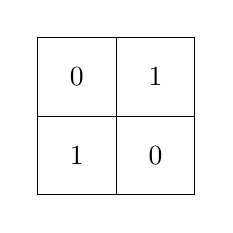
\begin{tikzpicture}

\tikzset{square matrix/.style={
		matrix of nodes,
		column sep=-\pgflinewidth, row sep=-\pgflinewidth,
		nodes={draw,
			minimum height=#1,
			anchor=center,
			text width=#1,
			align=center,
			inner sep=0pt
		},
	},
	square matrix/.default=1cm
}
%|[fill=yellow]|
\matrix[square matrix]
{
	0 & 1 \\
	1 & 0  \\
}; 
\end{tikzpicture}, \ \ B = 
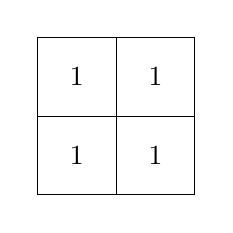
\begin{tikzpicture}

\tikzset{square matrix/.style={
		matrix of nodes,
		column sep=-\pgflinewidth, row sep=-\pgflinewidth,
		nodes={draw,
			minimum height=#1,
			anchor=center,
			text width=#1,
			align=center,
			inner sep=0pt
		},
	},
	square matrix/.default=1cm
}
%|[fill=yellow]|
\matrix[square matrix]
{
	1 & 1 \\
	1 & 1  \\
}; 
\end{tikzpicture}$$
$MI(A,B) = 0$, as the structures are very different.
Example 4:$$A = 
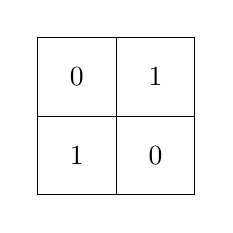
\begin{tikzpicture}

\tikzset{square matrix/.style={
		matrix of nodes,
		column sep=-\pgflinewidth, row sep=-\pgflinewidth,
		nodes={draw,
			minimum height=#1,
			anchor=center,
			text width=#1,
			align=center,
			inner sep=0pt
		},
	},
	square matrix/.default=1cm
}
%|[fill=yellow]|
\matrix[square matrix]
{
	0 & 1 \\
	1 & 0  \\
}; 
\end{tikzpicture}, \ \ B = 
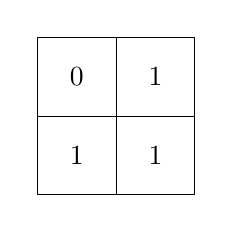
\begin{tikzpicture}

\tikzset{square matrix/.style={
		matrix of nodes,
		column sep=-\pgflinewidth, row sep=-\pgflinewidth,
		nodes={draw,
			minimum height=#1,
			anchor=center,
			text width=#1,
			align=center,
			inner sep=0pt
		},
	},
	square matrix/.default=1cm
}
%|[fill=yellow]|
\matrix[square matrix]
{
	0 & 1 \\
	1 & 1  \\
}; 
\end{tikzpicture}$$
$MI(A,B) = 0.32$\\
Keep in mind that $MI\geq0$, but can go up to 100 for large images!
\subsection{Calculating $P_A$, $P_B$, $P_{A,B}$}
Just create a table, then divide the right hand side by the amount of pixels/voxels:\\
$$\begin{tabular}{l|l}
	\hline
	0 & number of Pixels in image $A$ with greylevel 0\\
	$\vdots$ & $\vdots$\\
	255 & number of Pixels in image $A$ with greylevel 255\\
\end{tabular}$$\\
Calculating $P_{A,B}$ is a little difficult:\\
$$\begin{tabular}{l|lll}
	& 0 $\dots$ & $i$ & $\dots$ 255\\
	\hline
	0 & & & \\ 
	$\vdots$ & & \vdots &\\
	$i$ & \dots &\# pixel pins with colors $i,j$ &\\
	$\vdots$ & & &\\
	255 & & & \\
\end{tabular}$$
There are 3 algorithms/methods for calculation:
\begin{itemize}
	\item[1.] \textbf{Nearest Neighbour (NN)}
	\item[2.] \textbf{Trilinear Interpolation (TI)}
	\item[3.] \textbf{Trilinear Partial Volume (TPV)}
\end{itemize}
  \section{Imaging}\label{sec:imaging}
  \subsection{Image Deformation}
  There are multiple applications:
  \begin{itemize}
  	\item Elastic Registration 
  	\item Distortion Correction
  \end{itemize}
\subsubsection{Bilinear Onterpolation}
Assume we have 2 adjacent grid points $u,v$. To get from $G'$ to $G$ we have to deform $u$ in x-direction by $du$. We obtain information for $w$ by \textbf{linear interpolation}. Same for the y-direction.\\
\textbf{Advantage:} \begin{itemize}
	\item Simplicity
	\item We will move all points to its goal $\implies$ Accuracy!
\end{itemize}
\textbf{Disadvantage:} \begin{itemize}
	\item Not smooth
\end{itemize}
\subsubsection{Cubic Spline Interpolation}
We define a correction polynomial, two variables $x,y$
$$a_0 + a_1x+a_2y+a_3xy+a_4x^2+a_5y^2+a_6xy^2+a_7x^2y+a_8x^3 + a_9y^3$$
$$b_0 + b_1x+b_2y+b_3xy+b_4x^2+b_5y^2+b_6xy^2+b_7x^2y+b_8x^3 + b_9y^3$$
We have our model: $(x_m,y_m)$ and our distorted points $(x_d,y_d)$.\\
We further assume, that $a$'s and $b$'s are variables, while $x,y$ are constant.\\
We set up $f$ as:
$$f = [(x_m,y_m)-(x_d,y_d)]^2$$
For $N$ grid points, we adjust $f$ to:
$$f = [(x_m^{(1)},y_m^{(1)})-(x_d^{(1)},y_d^{(1)})]^2 + \dots + [(x_m^{(N)},y_m^{(N)})-(x_d^{(N)},y_d^{(N)})]^2$$
With $x_d$ being the $a$-Polynomial and $x_m$ being the $b$-Polynomial, function $f$ is quadratic in the $a$'s and $b$'s.
  \section{Motion Replication}\label{sec:motion}

\end{document}
